\documentclass[11pt, letterpaper]{article}

\usepackage{color}
\usepackage{fullpage}
\usepackage{graphicx}
\usepackage{hyperref}

\graphicspath{ {./img/} }

\begin{document}

\title{Introduction to UL Group 2 Safe Lock Manipulation}
\author{Grain ORice}
\date{April 2021\\
  {\color{blue}v0.5}}
\maketitle

\section*{License}
Copyright (C)  2021  Grain ORice

\noindent Permission is granted to copy, distribute and/or modify this document
under the terms of the GNU Free Documentation License, Version 1.3
or any later version published by the Free Software Foundation;
with no Invariant Sections, no Front-Cover Texts, and no Back-Cover Texts.
A copy of the license is included in the section entitled
``GNU Free Documentation License''.

\section*{About}

\begin{center}
  
\includegraphics[scale=.5]{lpu}
\end{center}

From \href{https://www.youtube.com/channel/UCHEPEHbo6kAxsxvIePE9kRw/about}{Lock
  Pickers United YouTube Channel} \\
Lockpickers United is a community of lockpickers from R/lockpicking on reddit
and the associated Discord channel. On this channel a handful of the black belt
pickers have come together to teach techniques, tools, and everything else to
new pickers as well as featuring detailed informational and pick videos of
extremely difficult locks. Please join us in enjoying the hobby, learning,
and progressing your skills and we do ours. More information and individual
pickers channels may be found on https://lockpickersunited.org though the site
is very new and needs significant work, we hope to build it and this channel
into solid resources for the community.
\newpage

\section*{Introduction}
\begin{center}
  \textbf{MANIPULATION \\
    \textit{Is the art of opening combination locks without the use of force
      or tools and in the absence of knowledge of the combination.}}
\end{center}

Locks and other security devices have relied on security through obscurity
throughout history as an integral part of the overall security model. This
peridium has been challenged by security experts, amateur lockpickers, and lock
enthusiasts recently. The art of manipulation was handed down between
locksmiths or other trusted individuals until the 20th century, when dedicated
classes were offered to teach this art. However, these classes were limited to
professionals and typically expensive. Information is available to anyone
interested, but most of the information is older works on the subject. There is
nothing wrong with the works available. The reader is encouraged to find such
materials and absorb the information presented. The concepts of manipulation
have not changed. The information provided in this document does not intend to
replace any professional works on the subject. The information provided is
intended for the locksport community and based on the community's information,
resources publicly available, and the author's practical knowledge.

Manipulation is the ability to gather information from the lock due to its
mechanical design and variations in mechanical tolerances. Just as in other
areas of locksport, the information is not necessarily hard to learn and
understand, but practice will be required to be proficient in the art of
manipulation. It's recommended to have good light and a quiet area to encourage
focused work when practicing. Manipulation uses sight, sound, and touch. The
better the reader's environment is to heighten these scenes, the better the
ability to learn manipulation. Later we will introduce reading the dial. It
will be imperative to maintain the same viewing angle when taking readings.

\noindent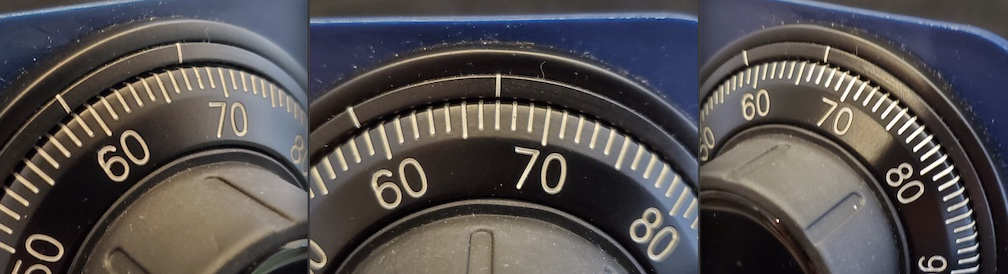
\includegraphics[width=\textwidth]{viewAngle}

\noindent The above image shows that looking at the dial face on shows a number
of '67'. However, when looked at from a different angle, the mark does not line
up directly with '67'. This example highlights why it is imperative to face the
dial from the same angle throughout the manipulation process.

The lock used in this document is a ``Big Red CDL-3'' manufactured by
\href{http://www.bigredsafelocks.com/Home-page/}{Big Red Safe Locks}. The
specific lock was purchased from \href{https://mbausa.com}{MBA USA Inc.} as a
pre-mounted cut-away training aid. The author does not have any business
connections with either of these companies and mentioned them for readers
interested in following along or looking for an affordable training lock to
learn manipulation.

When we talk about group 2 manipulation, we refer to safe locks certified by
Underwriters Laboratories (UL) under their UL 768 security rating. The UL 768
defines four levels of classification for mechanical safe locks. They are:
\begin{itemize}
  \item{Group 2}
  \item{Group 2M}
  \item{Group 1}
  \item{Group1R}
\end{itemize}

Some of the key properties of a group 2 safe lock are:
\begin{itemize}
  \item{1,000,000 theoretical combinations}
  \item{20 min of resistance to manipulation by a ``semi-skilled'' person.}
  \item{Has a re-locker.}
  \item{$\pm$1.25 dial number tolerance for three-wheel locks.}
  \item{$\pm$1.5 dial number tolerance for four-wheel locks.}
\end{itemize}

\section*{Nomenclature}
Before continuing, we will explore the common group 2 safe lock design and
identify the pieces that make up these locks.

\subsection*{Lock Case and Re-Locker}
The housing is where all the parts live to actuate the lock. In this
housing is the parts that we will be focusing on for manipulation.
The brass piece is the re-locker. When the case cover is removed, the
re-locker under spring tension will keep the bolt from retracting.

\begin{center}
  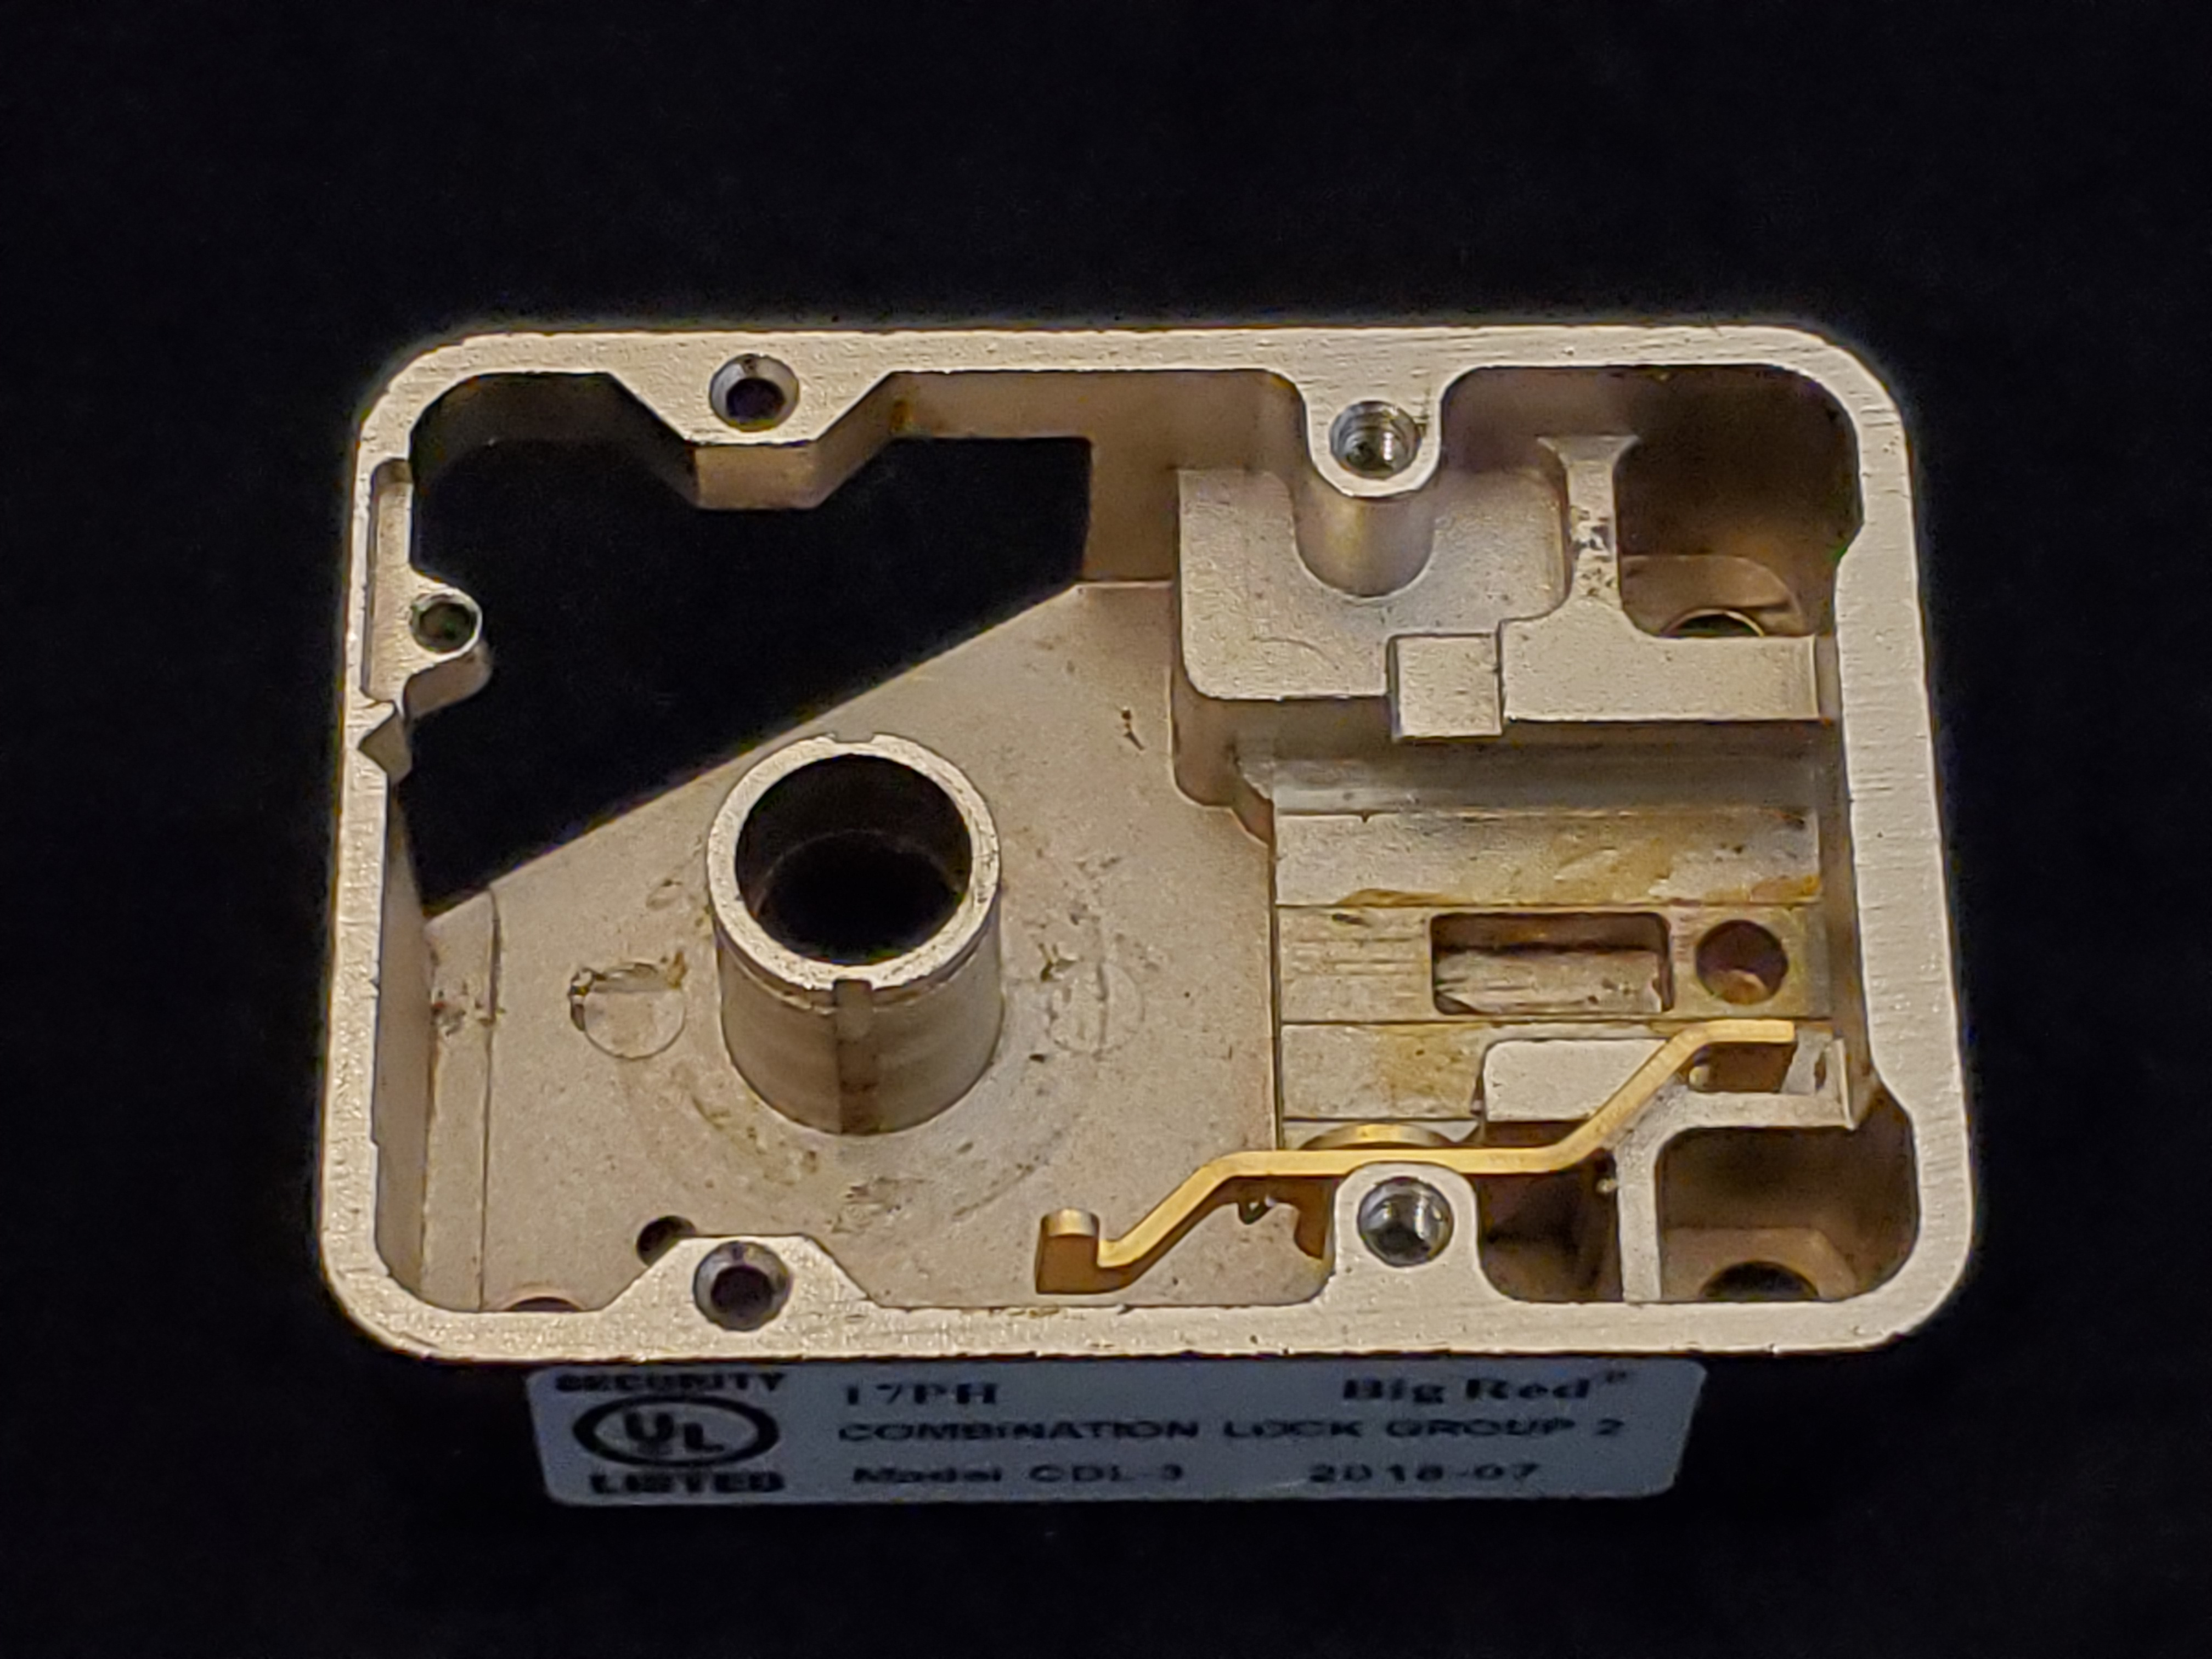
\includegraphics[scale=.075]{lockCase}
\end{center}

\subsection*{Case Cover}
The case cover is the service access to the lock. The case cover also has a line
near the center where the case cover can be broken. In the past, the dial could
be removed, and a would-be thief could punch out the case cover and allowing for
a device to be used to figure out the combination of the lock. The brake-away
line in the case cover would allow the back of the case to be punched away from
the Lock case. However, the re-locker under spring tension would lock the bolt
in place still covered by the remaining part of the case cover.

\begin{center}
  \includegraphics[scale=.075]{caseCover}
\end{center}

\subsection*{Dial Assembly}
In the following figure, we see the dial, which is the user interface to the lock.
Attached to the dial is the spindle, a threaded rod that attaches the dial to the
drive cam. The drive cam is a brass piece with markings on it. This marking
indicates where the spline key (metal L-shaped piece) is inserted based on the
lock's mounting position. Also pictured are the dial plate and a white bushing.

\begin{center}
  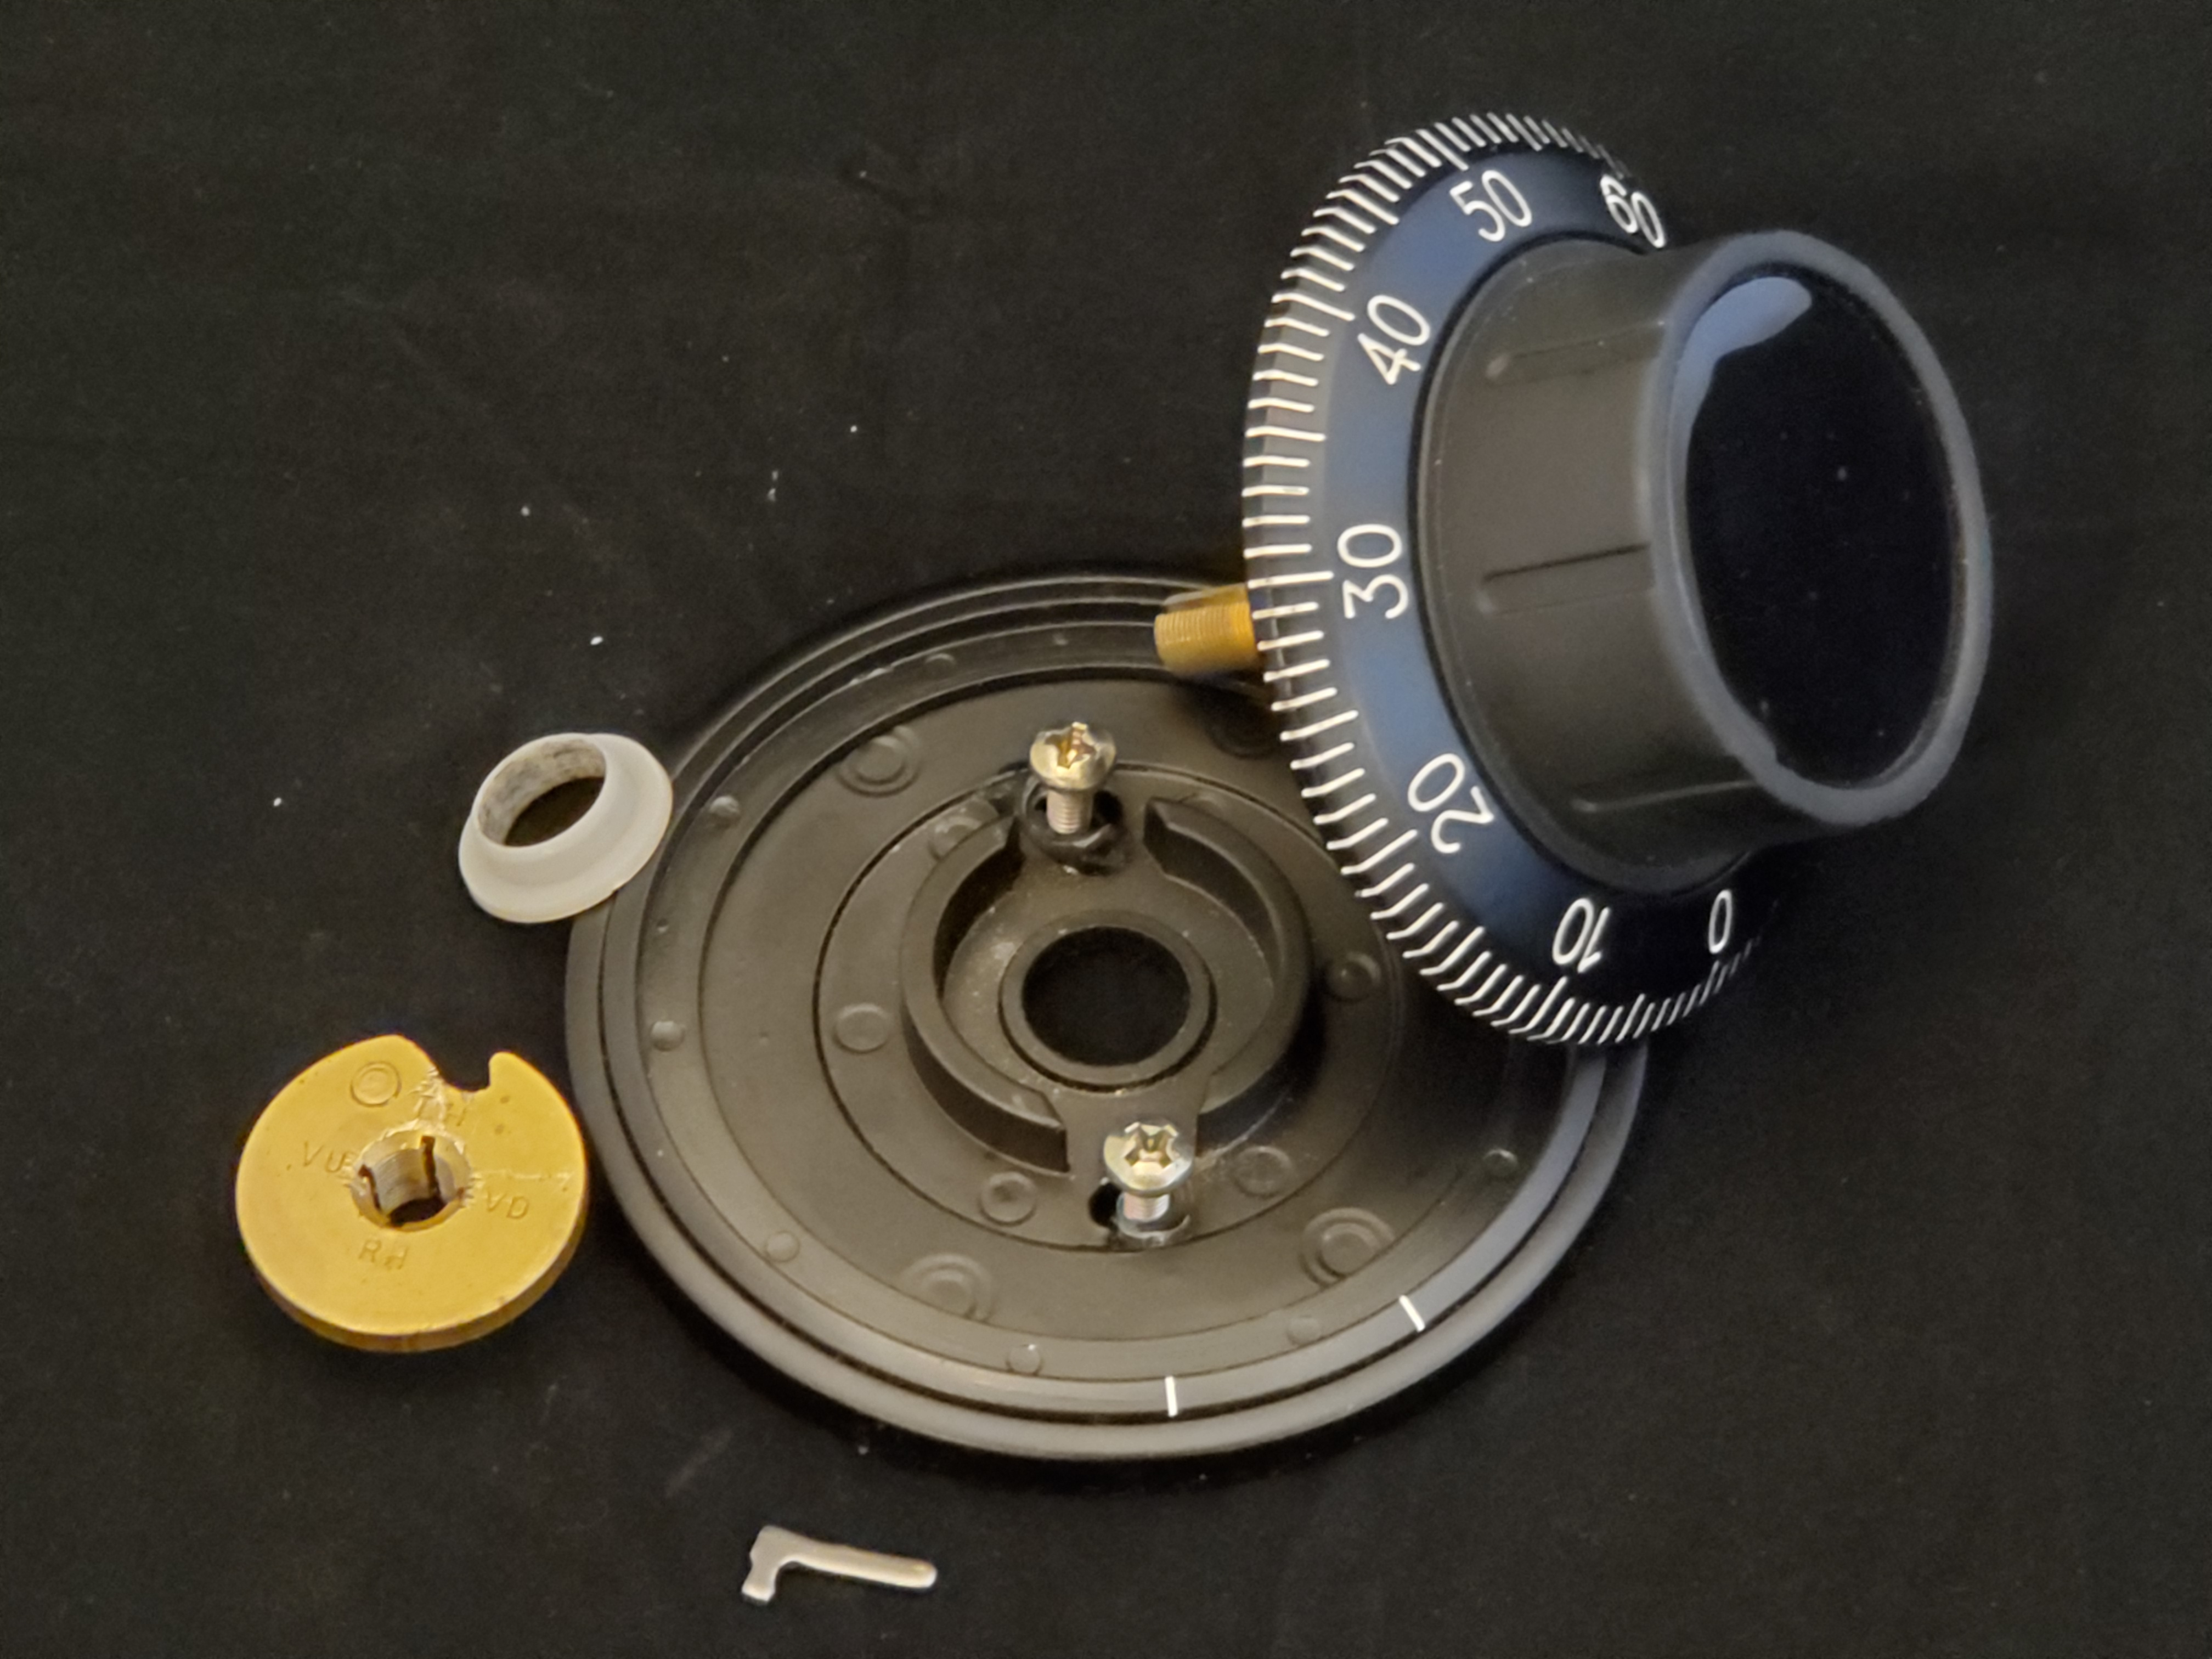
\includegraphics[scale=.075]{dialAssem}
\end{center}

\end{document}
